\usepackage[T1]{fontenc} % Codificación de las fuentes utilizadas
\usepackage[spanish]{babel} % Español como idioma principal del texto (permite hyphenation de palabras al final de una línea)


\usepackage{graphicx}
\usepackage{url}

\graphicspath{{Figures/}{Diagrams}{Chapters/}}  % Location of the graphics files (set up for graphics to be in PDF format)

\selectlanguage{spanish}

\setcounter{tocdepth}{1}

% Include any extra LaTeX packages required
\usepackage[square, numbers, comma, sort&compress]{natbib}  % Use the "Natbib" style for the references in the Bibliography
\usepackage{verbatim}  % Needed for the "comment" environment to make LaTeX comments
\usepackage{vector}  % Allows "\bvec{}" and "\buvec{}" for "blackboard" style bold vectors in maths
\hypersetup{urlcolor=blue, colorlinks=true}  % Colours hyperlinks in blue, but this can be distracting if there are many links.
\usepackage{hyperref}
% \usepackage[pdfauthor={Diego Martín Arroyo},
%             pdftitle={Diseño e implementación de un sistema de computación distribuida con
% Raspberry Pi, y estudio comparativo del mismo frente a otras soluciones},
%             pdfsubject={Memora del Trabajo de Fin de Grado},
%             pdfproducer={XeLaTeX with hyperref},
%             pdfcreator={XeLaTeX},
%             pdfkeywords={Computación Paralela, Sistema Distribuido, Raspberry}
%             ]{hyperref}
%% ----------------------------------------------------------------

%% --------------------------------------------------------------------------------------------------------------------------------
%http://tex.stackexchange.com/a/85218/76599
\usepackage{fancyvrb}
\usepackage[dvipsnames]{xcolor}

% redefine \VerbatimInput
\RecustomVerbatimCommand{\VerbatimInput}{VerbatimInput}% Inclusión de archivos de texto plano
{fontsize=\footnotesize,
 %
 frame=lines,  % top and bottom rule only
 framesep=2em, % separation between frame and text
 rulecolor=\color{Gray},
 %
 label=\fbox{\color{Black}data.txt},
 labelposition=topline,
 %
 commandchars=\|\(\), % escape character and argument delimiters for
                      % commands within the verbatim
 commentchar=*        % comment character
}

\usepackage{listings} % Requerido para la inserción de código
%Listings command

\usepackage{float}
\newcommand*\lstinputpath[1]{\lstset{inputpath=#1}}
\lstinputpath{Code/}

\newcounter{undefinedreferences}
\setcounter{undefinedreferences}{0}

\newcommand{\citationneeded}[1][None]{\stepcounter{undefinedreferences}\textsuperscript{\color{blue} [Citation needed: #1]}}

\newcommand{\checkreferences}{
\ifnum\value{undefinedreferences} > 0
\begin{center}
\immediate\write18{wget -O Figures/protester.png -nc http://imgs.xkcd.com/comics/wikipedian_protester.png}
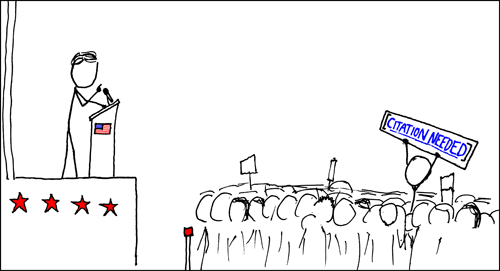
\includegraphics[width=\textwidth]{protester.png}\\
There are \arabic{undefinedreferences} undefined references
\end{center}
\else
No undefined references. Good!
\fi
}


%https://github.com/pads-fhs/LaTeX-Template-Thesis/blob/master/lststyles.tex
\lstdefinelanguage{JavaScript}{
  keywords={typeof, new, true, false, catch,%
    function, return, null, catch, switch, var,%
    if, in, while, do, else, case, break},
  ndkeywords={class, export, boolean, throw, implements, import, this},
  sensitive=false,
  comment=[l]{//},
  morecomment=[s]{/*}{*/},
  morestring=[b]',
  morestring=[b]"
}
\newcommand{\lstsetjavascript}{
  \lstset{
		language=JavaScript,
		breaklines=true,
		commentstyle=\textit,
		basicstyle=\ttfamily,
		keywordstyle=\bfseries,
		stringstyle=\ttfamily,
		showstringspaces=false,
		frame=single,
		tabsize=2
  }
}

\lstdefinelanguage{log}{
  keywords={typeof, new, true, false, catch,%
    function, return, null, catch, switch, var,%
    if, in, while, do, else, case, break},
  ndkeywords={class, export, boolean, throw, implements, import, this},
  sensitive=false,
  comment=[l]{//},
  morecomment=[s]{/*}{*/},
  morestring=[b]',
  morestring=[b]"
}
\newcommand{\lstsetlog}{
  \lstset{
		language=log,
		breaklines=true,
		commentstyle=\textit,
		basicstyle=\ttfamily,
		keywordstyle=\bfseries,
		stringstyle=\ttfamily,
		showstringspaces=false,
		frame=single,
		tabsize=2
  }
}

\lstloadlanguages{Java,XML, JavaScript, log}

\newcommand{\javascriptcode}[4]{
	\lstinputlisting[caption=#2,label=#1, firstline=#3, lastline=#4]{#1.json}
}

\newcommand{\logcode}[4]{
	\lstinputlisting[caption=#2,label=#1, firstline=#3, lastline=#4]{#1.log}
}

\usepackage[bottom]{footmisc} %The footnotes go at the bottom of t\usepackage{dtklogos}he page, instead next to the last line.
%Ajustes para Java
% \lstset{
% 	language=java,
%  	frame=single, % Un marco simple alrededor del código
%     basicstyle=\small\ttfamily, % Utilizar fuente true type pequeña
%     keywordstyle=[1]\color{Blue}\bf, % Funciones en negrita y azul
%     keywordstyle=[2]\color{Purple}, % Argumentos en morado
%     keywordstyle=[3]\color{Blue}\underbar, % Funciones personalizadas subrayadas en azul
%     identifierstyle=, % Nada especial acerca de identificadores
%     commentstyle=\usefont{T1}{pcr}{m}{sl}\color{Green}\small, % Los comentarios se renderizan en fuente pequeña verde
%     stringstyle=\color{Purple}, % Cadenas en morado
%     showstringspaces=false, % No se muestran los espacios entre cadenas
%     tabsize=5, % 5 espacios por tabulado
%     %
%     % Put standard Perl functions not included in the default language here
%     %morekeywords={rand},
%     %
%     % Put Perl function parameters here
%     %morekeywords=[2]{on, off, interp},
%     %
%     % Put user defined functions here
%     %morekeywords=[3]{test},\usepackage{dtklogos}
%    	%
%     morecomment=[l][\color{Blue}]{...}, % Line continuation (...) like blue comment
%     numbers=left, % Número de línea a la izquierda
%     firstnumber=1, % Número de línea comienza en 1
%     numberstyle=\tiny\color{Blue}, % Los números de línea son azules y pequeños
%     stepnumber=5, % Los números de línea van de 5 en 5
%     breaklines=true % Salto de línea si el texto no entra. See http://stackoverflow.com/a/1875803
% }

%\usepackage{xltxtra} % XeLaTeX logo. Yep, just that
%http://tex.stackexchange.com/a/73179/76599
\usepackage{metalogo}
%\usepackage{dtklogos} %BibTeX logo
\def\BibTeX{{\rm B\kern-.05em{\sc i\kern-.025em b}\kern-.08em
    T\kern-.1667em\lower.7ex\hbox{E}\kern-.125emX}}

\newenvironment{alignedDescription}[2][0pt]
  {\begin{list}{}%
    {\renewcommand\makelabel[1]{\textsf{\textbf{##1}}\hfil}%
     \settowidth\labelwidth{\makelabel{#2}}%
     \setlength\leftmargin{\labelwidth+\labelsep + #1}}}%
  {\end{list}}

\newenvironment{elements}
{\begin{quote}\itshape\centering\small}
{\end{quote}}

\newenvironment{cabstract}
{\begin{quote}\itshape\centering\small}
{\end{quote}}

%\usepackage[xindy]{glossaries}
%\newcommand{\chapterabstract}{1}{
%	\begin{center}
%	\small\textit
%	#1
%	\end{center}
%}

\usepackage{xcolor,colortbl}

\newcommand{\hmwkTitle}{Evaluación de herramientas} % Assignment title
\newcommand{\hmwkDueDate}{Martes,\ 28\ de\ April\ de\ 2015} % Due date
\newcommand{\hmwkClassInstructor}{Rodrigo Santamaría} % Teacher/lecturer
\newcommand{\hmwkAuthorName}{Diego Martín Arroyo} % Your name
\newcommand{\hmwkSubject}{2} % Evaluation subject number

%----------------------------------------------------------------------------------------
%   TITLE PAGE
%----------------------------------------------------------------------------------------

\title{\hmwkTitle\\Sujeto de evaluación n\hspace{-1.5mm}$\phantom{a}^{\circ}$ \hmwkSubject}
\author{\textbf{\hmwkAuthorName}}
\date{28 de abril de 2015} % Insert date here if you want it to appear below your name

\begin{document}
\maketitle

\tableofcontents
\section{Descripción}

\begin{itemize}
	\item \textbf{Perfil}: Estudiante de la asignatura \textbf{Sistemas Distribuidos}.
	\item No conocía las herramientas previamente.
\end{itemize}

\section{Introducción}

A medida que las herramientas desarrolladas maduran, es necesario realizar una evaluación de las mismas en una situación cada vez más próxima a un caso de uso ``real''. En la presente evaluación se realiza la integración de las herramientas con un sujeto que desea utilizar el sistema para realizar una práctica de la asignatura \textbf{Sistemas Distribuidos}, que requiere el uso de varios equipos que ejecuten una instancia del contenedor \textbf{Apache Tomcat} sobre los cuales se realizará el despliegue. Para ello, se proponen como alternativas a las herramientas utilizadas actualmente el siguiente conjunto:

\begin{itemize}
	\item \textbf{Deployer} para la realización del despliegue.
	\item \textbf{Status monitor} para conocer la información de cada nodo.
\end{itemize}

\section{Secuencia de pasos}

La evaluación es en este caso guiada: el sujeto realiza las acciones solicitadas por el evaluador y se le pregunta por la experiencia de uso en el desarrollo de las mismas.

\subsection{Paso 1: Planteamiento}

La evaluación comienza con un diálogo introductorio. Se describe la herramienta \textbf{Deployer}, sus características y potenciales aplicaciones para el caso concreto del sujeto.

En primer lugar se accede a la interfaz web del \textbf{Deployer}, indicando al usuario unas credenciales con las que acceder. Se le indica que en futuras versiones el acceso al sistema se realizará con las credenciales del sistema de usuarios propio de la infraestructura. Esta característica es valorada positivamente por el usuario.


\subsection{Paso 2: Toma de contacto con el sistema}

El sujeto comprende sin ayuda el funcionamiento de la interfaz. Sin embargo, pregunta cómo puede subir varios archivos a la vez. Esta característica ya está implementada, por lo que se indica al usuario cómo realizarlo.\\

Observa que al pasar varios segundos aparecen los equipos sobre los que puede realizar el despliegue. Sugiere utilizar una animación de progreso para indicar que aún falta información por aparecer.\\

El sujeto considera que la información que da la interfaz es suficiente para sus necesidades. Al plantearse mejoras tales como conocer qué servicios tiene cada nodo a través de la interfaz el usuario responde positivamente.\\

El sujeto indica que los selectores de cada nodo deben ser más intuitivos, pues a primera vista no era capaz de identificar su funcionalidad. Sugiere utilizar cuadros de alerta en caso de que ningún nodo haya sido seleccionado (actualmente el botón de despliegue se limita a no reaccionar) y modificar la lista de nodos a fin de incluir una casilla de selección en lugar del cambio de color como método de selección.

Al arrastrar varios ficheros, se indica al usuario de que únicamente es posible añadir un fichero por cada vez. El sujeto exige mejoras al respecto. %Este es un error del evaluador

Una vez ha arrastrado los archivos a desplegar, valora positivamente la interfaz de subida, en particular la posibilidad de ejecutar un comando antes de realizar el despliegue, y el hecho de que el alcance de dicha funcionalidad no esté limitado a la capacidad que cada usuario tiene al acceder de forma directa al equipo. También aprecia la información recibida por parte del sistema, que utiliza barras de progreso para indicar el estado de la subida.\\

Un problema a corregir gracias a esta evaluación es el hecho de que Tomcat no realiza el despliegue de los servicios de forma automática.\\

Otra de las ventajas que el sujeto sugiere añadir es un botón que permita evitar cualquier tipo de sobreescritura al desplegar nuevos ficheros. Bastaría en su opinión con una casilla de confirmación, que en su opinión puede estar por defecto marcada, dado que no suele sufrir problemas de pérdida de información por sobreescritura.\\

Se plantea la posibilidad de disponer de una interfaz por consola que complemente a la interfaz web que se ha planteado al usuario. Valora positivamente la propuesta, aunque considera suficiente la interfaz web.\\

\subsection{Paso 3: Ejecución}

El usuario puede acceder a su cuenta por SSH para ejecutar un comando (aunque podría haberlo realizado a través del \textbf{Deployer}, prefiere realizarlo de esta forma, pues desea conocer la salida por pantalla de la ejecución, algo que no es posible observar a través de la interfaz web). Se le sugiere utilizar una pequeña interfaz que muestre este tipo de mensajes para facilitar la depuración y su parecer es positivo.

Una vez ejecutado el proceso se le muestra al usuario la aplicación \textbf{Status Monitor}. El sujeto considera apropiada toda la información presente y no echa de menos información que pueda ser de su interés. Ante la sugerencia de una vista global de todos los nodos, coincide en que podría ser de utilidad. También afirma que sería útil unificar esta herramienta con el \textbf{deployer}, conociendo, por ejemplo, el número de recursos libres en cada máquina para hacer un despliegue que sature menos a un nodo.

\subsection{Paso 4: Otras herramientas}

Además de las herramientas ya evaluadas, se describen otras de las herramientas creadas, con objeto de conocer la opinión al respecto de las mismas (la evaluación de estas no fue llevada a cabo por problemas de tiempo).

\begin{itemize}
	\item Valora de forma muy positiva la herramienta \textbf{marcoinstallkey}.
	\item Considera que \textbf{marcosshcommand} puede servirle.
\end{itemize}

\section{Conclusiones}
De esta evaluación se sacan las siguientes conclusiones y acciones a llevar a cabo.
	\begin{itemize}
	\item En general, la experiencia de uso de este sujeto ha sido agradable y considera de utilidad las herramientas.
	\item Mejor intuitividad al subir varios archivos: Permitir que el sistema clasifique las entradas y cree una entrada en la lista de archivos a subir por cada entrada.
	\item Añadir una animación de carga mientras que \textbf{MarcoPolo} retorna la información sobre los nodos.
	\item Añadir una lista de los servicios ofertados por cada máquina.
	\item Crear un selector de nodos más intuitivo, aprovechando recursos ya conocidos por el usuario.
	\item Crear una herramienta que permita observar remotamente ficheros de \textbf{log}.
	\item Solucionar los problemas de recarga de Tomcat.
	\item Solucionar pequeños problemas en la disposición de elementos de la página.
	\end{itemize}
\end{document}